\documentclass[12pt]{beamer}

\usepackage[english]{babel}
\usepackage[T1]{fontenc}
\usepackage[utf8]{inputenc}
\usepackage{enumitem, tikz, chronosys}

\setitemize{
  itemsep=1em,
  label=\usebeamerfont*{itemize item}
    \usebeamercolor[fg]{itemize item}
    \usebeamertemplate{itemize item}
}

\usetikzlibrary{positioning, decorations.markings}
\tikzset{small/.style={draw,fill,circle,inner sep=1pt,outer sep=0pt}}

\setbeamertemplate{footline}[frame number]{}
\setbeamertemplate{navigation symbols}{}

% https://tex.stackexchange.com/a/167423
\newcommand{\backupbegin}{
  \newcounter{framenumberappendix}
  \setcounter{framenumberappendix}{\value{framenumber}}
}
\newcommand{\backupend}{
  \addtocounter{framenumberappendix}{-\value{framenumber}}
  \addtocounter{framenumber}{\value{framenumberappendix}}
}

\title{Reduction of Key Sizes on Rainbow-like Multivariate Signature Schemes}
\author{Gustavo Zambonin}
\institute{
  
\includegraphics[scale=0.15]{ufsc}                    \\ \vspace{-4mm}
  INE410111 --- Research Methodology in Computer Science \\ \vspace{2mm}
  \texttt{gustavo.zambonin@posgrad.ufsc.br}
}
\date{}

\begin{document}

\catcode`\@=11
\def\chron@selectmonth#1{\ifcase#1\or Jan\or Feb\or Mar\or Apr\or%
  May\or Jun\or Jul\or Aug\or Sep\or Oct\or Nov\or Dec\fi}

\begin{frame}[plain,noframenumbering]
  \titlepage
\end{frame}

\begin{frame}
  \frametitle{Context}
  \begin{itemize}
    \item Guarantee protection and privacy of messages sent digitally
    \item Security of digital signature schemes is based on problems from
        number theory
    \item There exist quantum algorithms~\cite{Shor:article:1997:oct} that
        solve these problems efficiently
    \item Post-quantum cryptography aims to create cryptosystems based on
        problems immune to quantum speedups
  \end{itemize}
\end{frame}

\begin{frame}
  \frametitle{Motivation}
  \begin{itemize}
    \item Imminent threat from quantum computers
    \item Several active branches of post-quantum cryptography
    \begin{itemize}
      \item Focus on cryptosystems that are based on the difficulty of solving
          systems of equations
    \end{itemize}
    \item Standardization calls by institutions such as NIST and IRTF
    \item Development of quantum computers by corporations, such as Google and
        Intel
  \end{itemize}
\end{frame}

\begin{frame}
  \frametitle{Multivariate cryptography}
  \begin{itemize}
    \item Cryptography based on systems of multivariate quadratic equations
        over finite fields
    \begin{figure}
      \vspace{2mm}
      \centering
      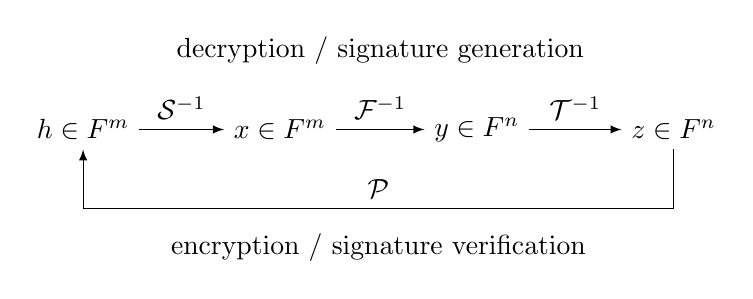
\begin{tikzpicture}
        \node (h) at (-2.5, 0) {$h \in \mathbb{F}^{m}$};
        \node (x) at (0, 0) {$x \in \mathbb{F}^{m}$};
        \node (y) at (2.5, 0) {$y \in \mathbb{F}^{n}$};
        \node (z) at (5, 0) {$z \in \mathbb{F}^{n}$};
        \draw[-latex] (h) -- (x) node[midway,above] {$\mathcal{S}^{-1}$};
        \draw[-latex] (x) -- (y) node[midway,above] {$\mathcal{F}^{-1}$}
          node[midway,yshift=1cm] {decryption / signature generation};
        \draw[-latex] (y) -- (z) node[midway,above] {$\mathcal{T}^{-1}$};
        \draw[-latex] (z) -- (5, -1) -- (-2.5, -1) node[midway,above]
          {$\mathcal{P}$} node[midway,yshift=-.5cm] {encryption / signature
          verification} -- (h);
      \end{tikzpicture}
    \end{figure}
    \item Fast operations, small signature sizes, large keys
  \end{itemize}
\end{frame}

\begin{frame}
  \frametitle{Underlying issue}
  \begin{itemize}
    \item Focus on the Rainbow signature scheme, due to Ding and
        Schmidt~\cite{Ding:inproc:2005:jun}, submitted to NIST for
          standardization
    \item Easy description, good balance between signature and key sizes
    \item Keys in the order of 10 KB, while classical schemes feature sub-1 KB
    \item Introduction of structures in the keys may lower security
  \end{itemize}
\end{frame}

\begin{frame}
  \frametitle{Related works}
  \begin{figure}[htbp]
    \tiny
    \startchronology[startyear=2010,stopyear=2018,startdate=false,
      stopdate=false,arrow=false,height=3pt]
    \chronoevent[markdepth=-50pt]{6/2010}{\cite{Petzoldt:inproc:2010:jun}}
    \chronoevent{12/2010}{\cite{Petzoldt:inproc:2010:dec}}
    \chronoevent[markdepth=-20pt]{3/2011}{\cite{Petzoldt:inproc:2011:mar}}
    \chronoevent[markdepth=40pt]{9/2011}{\cite{Petzoldt:inproc:2011:sep}}
    \chronoevent[markdepth=-50pt]{2/2012}{\cite{Yasuda:inproc:2012:feb}}
    \chronoevent{11/2012}{\cite{Petzoldt:inproc:2012:nov}}
    \chronoevent[markdepth=70pt]{5/2013}{\cite{Yasuda:inproc:2013:may}}
    \chronoevent[markdepth=-20pt]{6/2013}{\cite{Petzoldt:inproc:2013:jun}}
    \chronoevent[markdepth=40pt]{7/2013}{\cite{Petzoldt:phd:2013:jul}}
    \chronoevent[markdepth=-50pt]{1/2014}{\cite{Yasuda:article:2014:jan}}
    \chronoevent{4/2014}{\cite{Yasuda:inproc:2014:apr}}
    \chronoevent[markdepth=-20pt]{9/2014}{\cite{Yasuda:article:2014:sep}}
    \chronoevent{12/2015}{\cite{Shim:inproc:2015:dec}}
    \chronoevent[markdepth=-50pt]{6/2017}{\cite{Peng:article:2017:jun}}
    \chronoevent{6/2017}{\cite{Szepieniec:inproc:2017:jun}}
    \chronoevent[markdepth=-20pt]{12/2017}{\cite{Beullens:inproc:2017:dec}}
    \stopchronology
  \end{figure}
\end{frame}

\begin{frame}
  \frametitle{Hypothesis}
  \begin{itemize}
    \item Works have reduced either private or public keys, separately
    \item Do there exist any restrictions in doing both at the same time?
    \item Is it possible to generate a structured public key from a similarly
        composed private key?
    \item Introduction of matrix symmetries as possible arrangements may lower
        security
  \end{itemize}
\end{frame}

\begin{frame}
  \frametitle{Objectives}
  \begin{itemize}
    \item Establishment of fit matrix structures to be introduced
    \item Measurement of security achieved by keys created with those matrices
    \item Development of a method in which private and public keys are
        structurally related
    \item Description of a new signature scheme with carefully chosen
        parameters for devices with distinct requirements
  \end{itemize}
\end{frame}

\begin{frame}
  \frametitle{Methodology}
  \begin{itemize}
    \item Review schemes that reduce key sizes, cryptanalysis of these, and
        study matrix-like symmetric structures
    \item Create an algorithm to generate a compact private-public key
        pair
    \item Apply currently known cryptanalytic methods to test security of
        signatures created by these keys
    \item Compare performance and security with related works
    \item Publish and present results through papers, dissertation etc.
  \end{itemize}
\end{frame}

\begin{frame}
  \frametitle{Expected results}
  \begin{itemize}
    \item Identify the relationship between matrix types and their effect on
        security
    \item Deep analysis on how to maintain structure when generating a key pair
    \item Present a Rainbow-like signature scheme that features reduction of
        private and public key sizes
    \item International collaboration and scientific contributions
  \end{itemize}
\end{frame}

\backupbegin
\begin{frame}[plain, allowframebreaks]
  \frametitle{References}
  \bibliographystyle{alpha}
  {\scriptsize \bibliography{\jobname}}
\end{frame}
\backupend

\end{document}
